\documentclass[a4paper, 11pt]{article}

\usepackage[T1]{fontenc}

\usepackage[hidelinks]{hyperref}
    \hypersetup{
        pdftitle={THORN-2 Technical Referance Manual},
        pdfauthor={aTan}
        }


\usepackage{svg}
\usepackage{graphicx}
\usepackage{capt-of}

\usepackage{amsmath}
\usepackage{cleveref}
\usepackage[table]{xcolor}
\usepackage{tabularx}
\usepackage{hhline}
\usepackage{listings}
\usepackage{booktabs}
\usepackage{enumitem}
\usepackage{subcaption}
\usepackage{circuitikz}

% Taken from https://gist.github.com/AntonLydike/e339c3c3a4dcab8bc3c620b3fa436cda
% Modified for comment font and to remove additional register definitions
\lstdefinelanguage[RISC-V]{Assembler}
{
alsoletter={.}, % allow dots in keywords
alsodigit={0x}, % hex numbers are numbers too!
morekeywords=[1]{ % instructions
    lb, lh, lw, lbu, lhu,
    sb, sh, sw,
    sll, slli, srl, srli, sra, srai,
    add, addi, sub, lui, auipc,
    xor, xori, or, ori, and, andi,
    slt, slti, sltu, sltiu,
    beq, bne, blt, bge, bltu, bgeu,
    j, jr, jal, jalr, ret,
    scall, break, nop
},
morekeywords=[2]{ % sections of our code and other directives
    .align, .ascii, .asciiz, .byte, .data, .double, .extern,
    .float, .globl, .half, .kdata, .ktext, .set, .space, .text, .word
},
morekeywords=[3]{ % registers
    zero, ra, sp, gp, tp, s0, fp,
    t0, t1, t2, t3, t4, t5, t6,
    s1, s2, s3, s4, s5, s6, s7, s8, s9, s10, s11,
    a0, a1, a2, a3, a4, a5, a6, a7,
},
morecomment=[l]{;},   % mark ; as line comment start
morecomment=[l]{\#},  % as well as # (even though it is unconventional)
morestring=[b]",      % mark " as string start/end
morestring=[b]'       % also mark ' as string start/end
}
\definecolor{mauve}{rgb}{0.58,0,0.82}
\lstset{
    numbers = left,
    basicstyle=\small\ttfamily,                   % very small code
    breaklines=true,                              % break long lines
    commentstyle=\small\color{green!50!black},    % comments are green
    keywordstyle=[1]\color{blue!80!black},        % instructions are blue
    keywordstyle=[2]\color{orange!80!black},      % sections/other directives are orange
    keywordstyle=[3]\color{red!50!black},         % registers are red
    stringstyle=\color{mauve},                    % strings are from the telekom
    identifierstyle=\color{teal},                 % user declared addresses are teal
    frame=l,                                      % black line on the left side of code
    language=[RISC-V]Assembler,                   % all code is RISC-V
    tabsize=4,                                    % indent tabs with 4 spaces
    showstringspaces=false                        % do not replace spaces with weird underlines
}


\usepackage[backend=biber, style=ieee]{biblatex}
    \addbibresource{./Bibs/Sources.bib}


\usepackage{tikz}

\usepackage{tikz-timing}
    \usetikztiminglibrary{advnodes}

\title{THORN-2 Technical Referance Manual}
\author{aTan}


\emergencystretch=1em


\begin{document}

    %Commands to print OLD formatted logos
    \newcommand{\oldlonglogo}{\textit{Thorn}-1}
    \newcommand{\oldlogo}{\textit{\TH}-1}

    %Commands to print formatted logos
    \newcommand{\longlogo}{\textit{Thorn}-2}
    \newcommand{\logo}{\textit{\TH}-2}
    \newcommand{\linksection}[1]{\hyperref[#1]{\S \nameref*{#1}}}

    %Defines the number of stages in the pipeline for easy changing
    \newcommand{\pipestages}{??? }

    \newcommand{\ramshort}{IS61WV6416}
    \newcommand{\ramname}{IS61WV6416DBLL-10TLI-TR}

    \newcommand{\clkfreq}{40 MHz}
    \newcommand{\clktime}{25 ns}

    \begin{titlepage}
        \maketitle
        \thispagestyle{empty}   %Hide pagenumber on titlepage
    \end{titlepage}

    \begin{abstract}
        This document is a technical reference for the \longlogo\ (Stylised: \logo)
            computer. The \logo\ is an RV64i compatable CPU and supporting system
            created largely from 74-series logic ships, with the goal of making a
            fully-pipelined system capable of very-high-speed execution.
            It also serves as a proof of [in]sanity for the creator.
    \end{abstract}
    \newpage


    \pagenumbering{roman}
    \tableofcontents
    \listoffigures
    \listoftables
    \lstlistoflistings
    \newpage


    \pagenumbering{arabic}
    \section{Introduction}\label{sec:Introduction}
        \longlogo\ is a RISC-V CPU, designed to be fully compatable with the RV64i (integer only)
            standard module as defined in the RISC-V Instruction Set Architecture 
            (RV-ISA) specification \cite{RVISA}. It is a fully-pipelined design
            with \pipestages parallel stages 
            (see \linksection{sec:Intro:Pipeline})
            with hazard avoidance (\linksection{sec:Intro:HazAvoid}) and 
            operand forwarding (\linksection{sec:Intro:OpFwd}).

        This project has some fairly nebulous goals, but the general idea is
            to learn how CPUs work internally and make something interesting.
            They are here itemised:
            
            \begin{itemize}
                \item Implement a RISC-V CPU
                \item Utilise as few non-74 series chips as possible (no FPGA)
                \item Design the circuitry "by hand"
                \item Achieve \textasciitilde 40 MHz operation
                \item Have fun :3
            \end{itemize}

        Please don't tell me I'm doing this inefficiently or that there article
            better ways to implement things - I'm well aware.

        \subsection{Pipelining}\label{sec:Intro:Pipeline}

            \subsubsection{Why \logo\ Differs From Classic RISC}

            The pipeline structure of \logo\ differs from the traditional RISC
                one in that there are several more stages. These can be grouped
                into largly the same functional blocks, but spread across more
                stages; a setup reached after much design work on \oldlonglogo.

            Classic RISC is split into five stages: Fetch, Decode, Execute, Memory 
                and Writeback; with every instruction passing through each stage 
                in turn (with the correct options set). In implementing this, I 
                decided to use SRAM to store the 32 registers and to avoid using 
                asynchronous SRAM. The latter decision was based on the false 
                assumption that this would make the control circuitry easier to 
                design and less error prone. 
                I maintained the Synchronous SRAM design for quite a while, getting 
                as far as designing the whole control circuit for the registers 
                and starting work on the ALU, but ran into problems with timings.

            The SRAM ic I had chosen - IS61NLP6432a \cite{IS61NLP6432a} - were 
                themselves pipelined at three stages: Assert, wait, Read/Write. 
                Each cycle of the CPU required three register accesses 
                (two reads and a write), which was possible to achieve if each 
                cycle was split into four phases, $\phi_{0}, \phi_{1}, \phi_{2}, 
                \phi_{3}$. This imposed the requirement that every pipeline
                stage in the CPU must take four cycles, which was insufficient
                for the ALU to perform a 64-bit addition \emph{and} perform
                conditional inversion of the second operand for subtraction and
                check conditions. Thus, I decided to go back to the drawing board 
                and start again.

            The current design of \logo's pipeline is based around the ALU,
                rather than the registers. I needed four stages to add numbers,
                plus two more to condition the inputs and outputs, giving six.
                Register accesses can be done in one step by using two copies
                of each register (a poor-man's dual-port RAM) which are written 
                to simultaniously on the rising edge of the clock; then
                separately read on the falling edge. Now using fast, 
                \emph{asynchronous} SRAM instead.

        \subsection{Hazard Avoidance}\label{sec:Intro:HazAvoid}

            In a pipelined system, there are frequently situations where one
                instruction depends on the result of its predecessor. In such
                a case, this results in a \textbf{Data Hazard} - what is contained
                in register X is out of date, and reading this will produce
                incorrect results.

            Another hazard comes in the case that a conditional branch is dependent
                on the outcome of a previous operation, resulting in a 
                \textbf{Control Hazard}. The CPU must either stall new instructions
                while the condition is evaluated, or speculatively execute code
                for either the "branch" or "no branch" condition and throw it out if
                needed.
            
            \subsubsection{Adding Stalls}\label{sec:Intro:HazAvoid:Stalls}

                In either hazard case, the simplest - albeit least efficient - 
                    solution is to inject NO-OPs (NOPs) after the Decode stage 
                    and only continue when there are no remaining hazards. 
                    It is, however, trivial to come up with example programs which 
                    result in more nops than executed instructions:

                \begin{lstlisting}[language={[RISC-V]Assembler}, frame=single,]
;Some silly code  :3c
add a0, a1, a2  ;Use a0 as tally
add a0, a0, a3
add a0, a0, a4
add a0, a0, a5  ;Add lots of numbers in turn
;...
                \end{lstlisting}

                When executing the above program, the CPU is forced to insert NOPs
                    between every instruction to allow the addition result to be fully
                    written back to \lstinline[language={[RISC-V]Assembler}]|a0| before
                    the next instruction is executed. A classic RISC-V architecture 
                    with this simple hazard avoidance would \emph{actually} execute
                    the code in Listing \ref{lst:Intro:HazAvoid:Stalls:ManyNOPs}

                \begin{lstlisting}[
                        label={lst:Intro:HazAvoid:Stalls:ManyNOPs},
                        caption={Worst case scenario for consecutive adds.},
                        captionpos=b,
                        language={[RISC-V]Assembler}, 
                        frame=single, 
                        float]
;Oops, all stalls  TwT
add a0, a1, a2  ;Use a0 as tally
nop             ;Execute in ALU
nop             ;Skip memory access
nop             ;Write result to a0
add a0, a0, a3  ;Next ADD is allowed to continue
nop
nop
nop
add a0, a0, a4
nop             ;Each nop represents
nop             ;   1 stall cycle
nop
add a0, a0, a5  ;Add lots of numbers in turn
;...
                \end{lstlisting}


                This effectively quarters the useful throughput of the CPU in the
                    worst case, though most of the time this isn't likely to occur.
                    Using this method, the number of NOPs scales linearly with the
                    number of stages in the pipeline, so there is strong incentive
                    to use a better system. Such a system should be able to feed
                    data from one stage to another in order to skip some of the
                    waiting.

            \subsubsection{Operand Forwarding}\label{sec:Intro:OpFwd}

                \textbf{Operand Forwarding} is one way to reduce the number of stall
                    cycles introduced with a pipelined system. Here, in the case that
                    an instruction needs data which has not yet been written to a
                    register, but \emph{is available within the pipeline}, that data
                    can be fed forwards early so fewer stalls need to be introduced.

                This method becomes very important the longer a pipeline becomes due
                    to a greater number of cycles before the completion of each
                    instruction: there is greater chance that a following instruction
                    is dependent on a previous one \emph{and} that data takes longer
                    to become available.

                Assuming the same code snipped as in 
                    \linksection{sec:Intro:HazAvoid:Stalls}, a perfect system of 
                    operand forwarding could reduce the number of NOPs to zero 
                    - i.e. what is written is executed exactly.

                In \longlogo\ however, there is an additional complication which arises
                    from the use of a pipelined ALU: the final result is made available
                    in chunks across multiple stages or, should conditions need
                    evaluation, only available after the final stage.

                %Consecutive adds thru piped ALU
                \begin{figure}
                    \centering
                    
                    \begin{tabularx}{\textwidth}{
                        |>{\centering\arraybackslash}X
                        |>{\centering\arraybackslash}X
                        |>{\centering\arraybackslash}X
                        |>{\centering\arraybackslash}X
                        |>{\centering\arraybackslash}X
                        |>{\centering\arraybackslash}X
                        |
                        }
                        
                        \hhline{------}
                        Invert? &Add 1  &Add 2  &Add 3  &Add 4  &Cond.  \\
                        \hhline{|-|-|-|-|-|-|}

                        \rowcolor{lightgray}
                        \cellcolor{violet!50!white}I2   &   &   &   &   &   \\  \hhline{|-|-|-|-|-|-|}

                        \rowcolor{lightgray}
                        \cellcolor{violet!20!white}I3   &\cellcolor{violet!50!white}I2 &   &   &   &   \\  \hhline{|-|-|-|-|-|-|}
                        
                        \rowcolor{lightgray}
                        \cellcolor{green!20!white}I4    &\cellcolor{violet!20!white}I3 &\cellcolor{violet!50!white}I2 &   &   &   \\  \hhline{|-|-|-|-|-|-|}
                        
                        \rowcolor{lightgray}
                        \cellcolor{green!50!white}I5    &\cellcolor{green!20!white}I4 &\cellcolor{violet!20!white}I3 &\cellcolor{violet!50!white}I2 &   &   \\  \hhline{|-|-|-|-|-|-|}
                        
                        \rowcolor{lightgray}
                            &\cellcolor{green!50!white}I5 &\cellcolor{green!20!white}I4 &\cellcolor{violet!20!white}I3 &\cellcolor{violet!50!white}I2 &   \\  \hhline{|-|-|-|-|-|-|}
                        
                        \rowcolor{lightgray}
                            &   &\cellcolor{green!50!white}I5 &\cellcolor{green!20!white}I4 &\cellcolor{violet!20!white}I3 &\cellcolor{violet!50!white}I2 \\  \hhline{|-|-|-|-|-|-|}
                        
                        \rowcolor{lightgray}
                            &   &   &\cellcolor{green!50!white}I5 &\cellcolor{green!20!white}I4 &\cellcolor{violet!20!white}I3 \\  \hhline{|-|-|-|-|-|-|}
                        
                        \rowcolor{lightgray}
                            &   &   &   &\cellcolor{green!50!white}I5 &\cellcolor{green!20!white}I4 \\  \hhline{|-|-|-|-|-|-|}
                        
                        \rowcolor{lightgray}
                            &   &   &   &   &\cellcolor{green!50!white}I5 \\  \hhline{|-|-|-|-|-|-|}

                        \hhline{------}
                        
                    \end{tabularx}
                    \caption{Execution flow through a pipelined ALU. $I_{n}$ refers 
                             to line number in code listing.}
                    \label{fig:Intro:OpFwd:ALUBehav}
                \end{figure}

                In \cref{fig:Intro:OpFwd:ALUBehav}, each of the \emph{Add} stages
                    performs a 16-bit addition of each \ttfamily int16 \normalfont 
                    chunk of the 64-bit inputs. If operand forwarding were to be 
                    used, the output of \emph{Add 1} would need to be fed back to 
                    its inputs for the next instruction.
                    The same would be needed for each subsequent stage too.
                    See \linksection{sec:ALU} for how this is actually done.

    \section{Program Counter}\label{sec:PC}

        The PC's job is (generally) to increment by 4 every clock cycle to fetch the
            next instruction in memory. On occasion, it will need to stall in place, 
            load a provided value, or add a constant to its previous value to branch.

        While outwardly simple, this is fairly complex to actually implement in 64 bits,
            expecially the branch operation which requires a 12-bit add, then a carry to 
            propagate up the remaining bits. Since there could realistically be any
            arbitray sequence of branches, jumps, normal increments or stalls, all of
            the separate branches need to be done in parallel and selected from at the
            very end.

        

    \section{Decode Logic}\label{sec:Decode}

    \section{Immediate Value Generator}\label{sec:ImVal}

    \section{Registers}\label{sec:Regs}
        
        RV64i specifies 32 64-bit general-purpose registers and a program counter, PC.
            x0 is hardwired to \verb|0x0000 0000 0000 0000|; there is no stack
            pointer. None of the registers are otherwise special, but do have expected
            uses as per the calling convention \cite{RV-CallConv}, 
            shown in \cref{tab:Regs:CallConv}

        %Calling convention table
        \begin{table}[htb!]
            \centering
            \caption{RISC-V calling convention}\label{tab:Regs:CallConv}
            
            \begin{tabularx}{\textwidth}{
                >{\hsize=0.15\hsize\raggedright\arraybackslash}X
                >{\hsize=0.20\hsize\raggedright\arraybackslash}X
                >{\hsize=0.35\hsize\raggedright\arraybackslash}X
                >{\hsize=0.30\hsize\raggedright\arraybackslash}X
                }
                
                \toprule
                
                Register    &ABI Mnemonic   &Meaning    &Preserved across calls?    \\
                
                \midrule\addlinespace

                x0      &zero   &Zero     &---(Immutable)  \\
                x1      &ra     &Return address     &No     \\
                x2      &sp     &Stack Pointer      &Yes    \\
                x3      &gp     &Global Pointer     &---(Unallocatable) \\
                x4      &tp     &Thread Pointer     &---(Unallocatable) \\
                x5-7    &t0-2   &Temp. Registers    &No     \\
                x8-9    &s0-s1  &Callee-saved regs. &Yes    \\
                x10-17  &a0-7   &Argument registers &No     \\
                x18-27  &s2-11  &Callee-saved regs. &Yes    \\
                x28-31  &t3-6   &Temp. Registers    &No     \\

                \bottomrule

            \end{tabularx}
        \end{table}

        As each register is effectively the same, they are most easily implemented
            using SRAM. Learning from \oldlonglogo, I have decided to use the
            IS61WV6416DBLL-10TLI-TR \cite{RegRAMChip}; it's a 
            64k x 16-bit asynchronous SRAM ic with a 10 ns access time and single
            3.3 V supply.

        \subsection{Theory of Operation}\label{sec:Regs:TheoryOp}
        
        For every RV64i operation, there are up to two operands, meaning up to two
            registers may be read each cycle. There may also be a value written into
            a register. 
            Since the \ramshort\ is not multi-port, two copies of the register file
            are required: \textbf{x} and \textbf{y}; these are both 
            written to and read from (at different addresses) at the same time.

            \begin{figure}[htb!]
                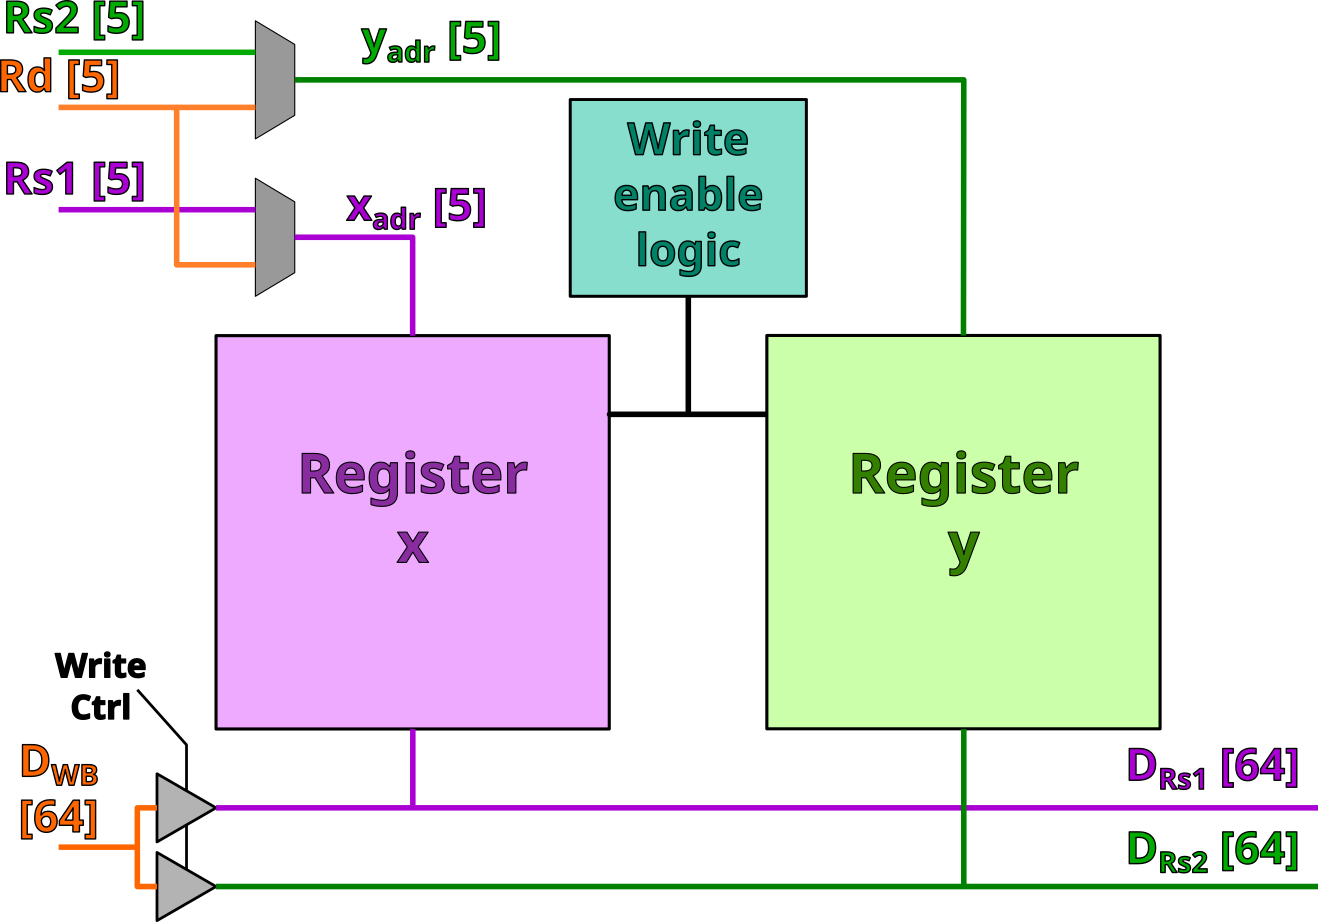
\includegraphics[width=\textwidth]{Figures/RegFile_TopLevel.png}
                \caption{The \longlogo\ register file.}
                \label{fig:Regs:TheoryOp:StdRegFile}
            \end{figure}

        Both access to \textbf{x} and \textbf{y} (Read/Write) occur within one cycle;
            writes are completed on the rising edge, $\phi_{1}$; and reads on the
            falling edge, $\phi_{2}$. Doing it in this order means neither the 
            writeback value, $D_{WB}$, nor the two read values, $D_{Rs1}$ and 
            $D_{Rs2}$, need additional latches - the former is latched from the output
            of the previous stage and the latter are latched on the next $\phi_{1}$.
            Some operations, such as conditional branches, compute a "result" which isn't
            needed. These instructions generate a write-blocking signal which prevents 
            the value $D_{WB}$ being committed to memory.

        \begin{figure}[htb!]
            \centering
            \begin{tikzpicture}[timing/picture]

                \timing[timing/unit=5mm, name=CLKTim] at (0,0) {0.5L N(T0) 3{H}N(T1) 3{L}N(T2) 3{H}N(T3) 3{L}N(T4) 0.5H}; 
                    \node[anchor=east](CLK_Label) at (CLKTim.west) {Clock};

                \timing[timing/unit=5mm, name=Adr1] at (0,-2.5) {0.5D{} 6{D}{01000} 6{D}{01001} 0.5D};
                    \node[anchor=east](Adr1_Label) at (Adr1.west) {Rs1 [5]};

                \timing[timing/unit=5mm, name=Adr2] at (0,-5.0) {0.5D{} 6{D}{01010} 6{D}{01011} 0.5D};
                    \node[anchor=east](Adr2_Label) at (Adr2.west) {Rs2 [5]};

                \timing[timing/unit=5mm, name=wAdr] at (0,-7.5) {0.5D{} 6{D}{11111} 6{D}{11110} 0.5D};
                    \node[anchor=east](wAdr_Label) at (wAdr.west) {Rd [5]};


                
                \timing[timing/unit=5mm, name=WrCtrl] at (0,-11.0) {0.5L L H L 9{L} 0.2H};
                    \node[anchor=east](WrCtrl_Label) at (WrCtrl.west) {Write};
                
                \timing[timing/unit=5mm, name=xAdr] at (0, -13.5) {0.5D{} 3{D}{11111} 3{D}{01000} 6{D}{01001} 0.5D};
                    \node[anchor=east](xAdr_Label) at (xAdr.west) {$\mathbf{x}_{addr}$};

                \timing[timing/unit=5mm, name=yAdr] at (0, -16.0) {0.5D{} 3{D}{11111} 3{D}{01010} 6{D}{01011} 0.5D};
                    \node[anchor=east](yAdr_Label) at (yAdr.west) {$\mathbf{y}_{addr}$};

                
                \timing[timing/unit=5mm, name=xData] at (0, -19.5) {0.5D{} 3D{$D_{WB, 1}$} 3D{$D_{Rs1, 1}$} 3D{$D_{WB, 2}$} 3D{$D_{Rs1, 2}$} 0.5D{}};
                    \node[anchor=east](xData_Label) at (xData.west) {$\textbf{D}_{Rs1}$ [64]};

                \timing[timing/unit=5mm, name=yData] at (0, -22.5) {0.5D{} N(B0) 3D{$D_{WB, 1}$}N(B1) 3D{$D_{Rs2, 1}$}N(B2) 3D{$D_{WB, 2}$}N(B3) 3D{$D_{Rs2, 2}$}N(B4) 0.5D{}};
                    \node[anchor=east](yData_Label) at (yData.west) {$\textbf{D}_{Rs2}$ [64]};

                \draw[green!75!red](T0.HIGH)+(0, 2.5) -- (B0.low) node[pos=0, anchor=north west, black]{\scriptsize Writeback enabled};
                \draw[red!50!blue](T2.HIGH)+(0, 2.5) -- (B2.low) node[pos=0, anchor=north west, black]{\scriptsize Writeback disabled};
                \draw[gray](T4.HIGH)+(0, 2.5) -- (B4.low) ;

                \node[anchor=south west] at (T0.low) {\footnotesize$\phi_{1}$};
                \node[anchor=south west] at (T1.low) {\footnotesize$\phi_{2}$};

                \node[anchor=south west] at (T2.low) {\footnotesize$\phi_{1}$};
                \node[anchor=south west] at (T3.low) {\footnotesize$\phi_{2}$};

            \end{tikzpicture}
            
            \caption{\longlogo\ register file timing diagram.}
            \label{tim:Regs:TheoryOp:RegTiming}
        \end{figure}

        \subsection{Control Logic}\label{sec:Regs:CtrlLogic}

            The design shown in \cref{fig:Regs:TheoryOp:StdRegFile} features two main
                elements which require "control logic" - the provided addresses, 
                $\mathbf{x}_{adr}$ and $\mathbf{y}_{adr}$, and control over the data
                busses, $\mathbf{D}_{Rs1}$ and $\mathbf{D}_{Rs2}$. In $\phi_{1}$, both
                are dedicated to the writeback operation and the read operation in
                $\phi_{2}$. This occurs \emph{whether or not} the write is needed, the
                only difference in the latter case being whether the \ramshort\ commits
                $\mathbf{D}_{WB}$ to storage (shown in \cref{tim:Regs:TheoryOp:RegTiming}).
            
            The write signal is generated by ANDing the write-enable signal (external)
                with a rising-edge detector on the clock line. When writeback is enabled
                this pulse occurs and is delayed enough for the address and data lines
                to settle.

    \section{ALU}\label{sec:ALU}

        The \longlogo\ ALU is comprised of three blocks - the Adder, Shifter and Logicer. 
            They do what their name suggests: the Adder computes $A \pm B$; the 
            Shifter shifts $A$ up or down by \textit{n} bits; and the Logic-er 
            performs the bitwise logic operations $A \cdot B$, $A + B$ and 
            $A \oplus B$. The 64-bit values $A$ and $B$ may be read from registers 
            or immediate values derived from an instruction. Each of the three blocks 
            are contained on separate circuit boards, but run in parallel. Their 
            outputs are calculated for all inputs with the relevant one forwarded to 
            the next pipeline stage.

        \subsection{Adder}\label{sec:ALU:Adder}
        
            The adder computes $A \pm B$ and optionally checks the result against each of 
                the "flags" for the calculation: $A < B$, $A = B$ and $A \ge B$. In 
                \oldlogo, this procedure was to be pipelined at up to six stages, but 
                this resulted in both huge pipelines and immense complications in feeding 
                partial results back to previous stages, possibly from multiple 
                instructions at multiple different points in their execution.
                In \logo, however, the entire ALU instead operates in one cycle - the 
                length of this defining the overall cycle length of the CPU. This is 
                also one of the few stages in the pipeline which needs non-74-series 
                chips.

            
            \subsubsection{Method}\label{sec:ALU:Adder:Method}

                Addition and subtraction are both done with the same circuitry, with a
                    pre-conditioning step for the second input, \textbf{B}. Using 
                    2's compliment to represent negative numbers, an $n$-bit number, $x$, 
                    can be negated by inverting its bits and adding 1:

                    \begin{equation}
                        -x := (x \oplus [2^{n}-1]) + 1
                    \end{equation}

                Subtracting \textbf{B} from \textbf{A} is therefore defined:

                    \begin{equation}\label{eq:ALU:Adder:SubDef}
                        \mathbf{A - B \ \equiv\ A + (-B) \ \equiv\ A + (B} \oplus [2^{n}-1]) + 1
                    \end{equation}

                \Cref{eq:ALU:Adder:SubDef} is implemented by passing \textbf{B} through
                    a bitwise XOR with the ADD/SUB setting, 
                    $\mathbf{K} = \overline{Add}/Sub$, and setting the carry input, 
                    $C_{in}$ to the same:

                    \begin{equation}
                        \mathbf{A - B \ \equiv\ A + (B \oplus [K]) + K}
                    \end{equation}

                The XORed \textbf{B} will be called $\mathbf{B'}$ from here.

                The addition, $\mathbf{A} + \mathbf{B'} + \mathbf{K}$ is a 64-bit
                    operation which would be much too slow if performed as a series of
                    daisy-chained segments due to the access time of the RAM ICs. Even
                    in the best case - where the access time were $\le 8$ ns - a chain of
                    eight in a row would be a total delay of $\le 64$ ns, greatly
                    bottlenecking the speed of the processor. A form of carry-lookahead
                    is therefore used to reduce this delay.

            \subsubsection{Modified Carry-Lookahead}\label{sec:ALU:Adder:ModCLA}
                    
                A traditional carry-lookahead circuit generates the carry signals from
                    chunks of the inputs, ideally much faster than the same signal would
                    be propagated up a chain of full adders. To do this, additional
                    signals are generated or tapped from the full adder circuits:
                    
                    \begin{align}
                        X_n   &= A_n \cdot B_n  \label{eq:ALU:Adder:ModCLA:X}   \\   
                        S_n   &= A_n \oplus B_n \label{eq:ALU:Adder:ModCLA:S}
                    \end{align}

                These additional signals are then used to calculate whether the \(n\)-bit
                    chunk generates, \textbf{G}, or propagrates, \textbf{P}, a carry.
                    An extra signal, \(\mathbf{Z}_n\) is used for checking conditions, 
                    see \linksection{sec:ALU:Adder:Conds}

                
                \begin{equation}\label{eq:ALU:Adder:ModCLA:G}
                    \mathbf{G}  =   (X_n) + 
                                    (X_{n-1} \cdot S_{n}) + 
                                    \dots + 
                                    \left( X_0 \cdot \prod_{i=1}^{n}(S_i) \right)
                \end{equation}

                \begin{equation}\label{eq:ALU:Adder:ModCLA:P}
                    \mathbf{P}  =   \prod_{i=0}^{n}(S_i)
                \end{equation}

                \begin{equation}\label{eq:ALU:Adder:ModCLA:Z}
                    \mathbf{Z}  = \begin{cases}
                        0 & \text{, } A + B \not\equiv 0 \pmod{255} \\
                        1 & \text{, } A + B \equiv 0 \pmod{255}
                    \end{cases}
                \end{equation}


                A single 64Kx8 RAM chip is used as a lookup table for \textbf{G} and 
                    \textbf{P}, and an additional output signals whether
                    \(\mathbf{A+B}=0\). \textbf{P} and \textbf{G} are then forwarded
                    to another 128Kx8 RAM which stands in for the combinotorial logic
                    which generates the carry signals.
                
                For \(n=0\):
                \begin{equation}\label{eq:ALU:Adder:ModCLA:C0}
                    C_0 = G_0 + C_{in} \cdot P_0
                \end{equation}

                For \(1 \le n < 8\):

                \begin{equation}\label{eq:ALU:Adder:ModCLA:Cn}
                    C_n =   G_n + 
                            \sum_{i=1}^{n}\left(G_{n-i} \cdot \prod_{j=0}^{i-1}\left(P_{n-j}\right)\right) +
                            C_{in}\cdot \prod_{N}\left(P_n\right)
                \end{equation}

                Using this method, all eight carrys can be generated after only two RAM
                    accesses.

            \subsubsection{Doing the Adding}\label{sec:ALU:Adder:Adding}

                The addition itself is "executed" in eight 128Kx8 RAM chips, each
                    programmed at start-up from a single 128Kx8 EEPROM. The RAM is
                    addressed by each byte of the two inputs, 
                    \(\mathbf{A}_{n}\) and \(\mathbf{B}_{n}\), and \(\mathbf{C}_{n}\), 
                    which points to the result, \(\mathbf{Y}_n\).

                \begin{table}[htb]
                    \centering
                    \caption{ALU adder EEPROM contents}
                    \label{sec:ALU:Adder:Structure:ramTab}
                    \begin{tabularx}{\linewidth}{X X X X X}
                        \addlinespace
                        \toprule
                        \(\mathbf{A}_n\)  &\(\mathbf{B}_n\) &\(\mathbf{C}_n\)   &Address  &\(\mathbf{Y}_n\) \\
                        \midrule
                        \addlinespace

                        0x00    &0x00   &0  &0x00000    &0x00   \\
                        0x00    &0x01   &0  &0x00001    &0x01   \\
                        \dots   &       &   &           &       \\
                        0x01    &0x00   &0  &0x00100    &0x01   \\
                        \dots   &       &   &           &       \\
                        0x00    &0x00   &1  &0x10000    &0x01   \\
                        \dots   &       &   &           &       \\
                        0xFF    &0xFE   &1  &0x1FFFE    &0xFE   \\
                        0xFF    &0xFF   &1  &0x1FFFF    &0xFF   \\

                        \bottomrule
                    \end{tabularx}
                \end{table}

                The final result is then either forwarded to the Adder's output, or
                    changed to 0/1 for the outcome of the SLT/SLTU instructions.

                In the case of ADDW/SUBW instructions which sign-extend a 32-bit answer
                    to 64, the upper word is ignored and switched to \textbf{Y}[31].

            \subsubsection{Condition Checking}\label{sec:ALU:Adder:Conds}

                The RISC-V ALU needs to be able to check for three conditions for both
                    signed and unsigned numbers: \(\mathbf{A < B}\), \(\mathbf{A = B}\)
                    and \(\mathbf{A \ge B}\). These are only valid if the calculation
                    \(\mathbf{A-B}\) was performed.
                    These checks can be performed immediately after the final carry 
                    out has been calculated using the equations in 
                    \cref{tab:ALU:Adder:Conds:ALUConds}.

                \begin{table}[htb]
                    \centering
                    \caption{Formulae for ALU result conditons}
                    \label{tab:ALU:Adder:Conds:ALUConds}
                    \begin{tabularx}{\textwidth}{X X X X}
                        \addlinespace
                        
                        \toprule
                        Condition   &Name   &Signed     &Unsigned   \\
                        \midrule \addlinespace

                        \(A < B\)   &LT &\(\overline{A_{63} \oplus B_{63}} \oplus C_{7}\)   &\(\overline{C_{7}}\)   \\
                        \(A = B\)   &EQ &\(Y = 0\)  &\(Y = 0\)  \\
                        \(A \ge B\) &GE &\(\overline{A < B}_S\) &\(C_7\)\\
                        \bottomrule
                    \end{tabularx}
                \end{table}

                The greater/less than checks are calculated as written, but the equality
                    check is actually calculated using the formula:

                \begin{equation}
                    EQ = \prod_{N}\left((P_{n} \cdot C_{in}) + (Z_{n} \cdot \overline{C_{in}})\right)
                \end{equation}

                In plain english: \(A\) and \(B\) are equal if the result of \(A - B\) is
                    zero. This occures when each 8-bit chunk, \(Y_n\), is equal to 0 with
                    no carry in, or is equal to 255 with a carry in.

                The results of the condition check are forwarded to the program counter
                    to deal with branches.


        \subsection{Logicer}\label{sec:ALU:Logicer}

            RISC-V specifies three bitwise logic operations: AND, OR and XOR. The most
                intuitive way to do this (74x08 for AND, 74x32 for OR, and 74x86 for XOR),
                takes 48 chips, plus some extra to choose which answer we want - quite a
                high number considering what this section does. This can be improved
                using a slightly more complex setup.

            The final output, \textbf{Y}, is sent to a tri-state buffer/line driver which
                is only enabled when the ALU performs a logic operation.

            \subsubsection{Logic from MUXs}\label{sec:ALU:Logicer:MUXLogic}

                It is possible to construct any 2-input, 1-output logic function from
                    a 4:1 MUX where the four inputs reflect the truth table of the
                    function, and the select lines are the two inputs of the function.

                Constructing the logic section this way means the control logic for this
                    section is limited to a small ROM containing the truth tables for the
                    MUXs.

                \begin{table}[htb]
                    \centering
                    \caption{Truth tables of the three defined logic operations}
                    \label{tab:ALU:Logicer:MUXLogic:TruthTab}
                    \begin{subtable}{0.3\textwidth}
                        \centering
                        \begin{tabularx}{\textwidth}{
                            >{\hsize=0.3\hsize\arraybackslash}X 
                            >{\hsize=0.3\hsize\arraybackslash}X 
                            >{\hsize=0.4\hsize\arraybackslash}X 
                            }
                    
                            \addlinespace\toprule

                            A   &B  &\(A \cdot B\)  \\  \midrule\addlinespace
                            0   &0  &0  \\
                            0   &1  &0  \\
                            1   &0  &0  \\
                            1   &1  &1  \\
                            \bottomrule
                    
                        \end{tabularx}
                        \caption{AND truth table}\label{tab:ALU:Logicer:MUXLogic:TruthTab:AND}
                    \end{subtable}
                    \hfill
                    \begin{subtable}{0.3\textwidth}
                        \centering
                        \begin{tabularx}{\textwidth}{
                            >{\hsize=0.3\hsize\arraybackslash}X 
                            >{\hsize=0.3\hsize\arraybackslash}X 
                            >{\hsize=0.4\hsize\arraybackslash}X 
                            }
                    
                            \addlinespace\toprule

                            A   &B  &\(A + B\)  \\  \midrule\addlinespace
                            0   &0  &0  \\
                            0   &1  &1  \\
                            1   &0  &1  \\
                            1   &1  &1  \\
                            \bottomrule
                    
                        \end{tabularx}
                        \caption{OR truth table}\label{tab:ALU:Logicer:MUXLogic:TruthTab:OR}
                    \end{subtable}
                    \hfill
                    \begin{subtable}{0.3\textwidth}
                        \centering
                        \begin{tabularx}{\textwidth}{
                            >{\hsize=0.3\hsize\arraybackslash}X 
                            >{\hsize=0.3\hsize\arraybackslash}X 
                            >{\hsize=0.4\hsize\arraybackslash}X 
                            }
                    
                            \addlinespace\toprule

                            A   &B  &\(A \oplus B\)  \\  \midrule\addlinespace
                            0   &0  &0  \\
                            0   &1  &1  \\
                            1   &0  &1  \\
                            1   &1  &0  \\
                            \bottomrule
                    
                        \end{tabularx}
                        \caption{XOR truth table}\label{tab:ALU:Logicer:MUXLogic:TruthTab:XOR}
                    \end{subtable}
                \end{table}

                \begin{figure}[htb]
                    \centering
                    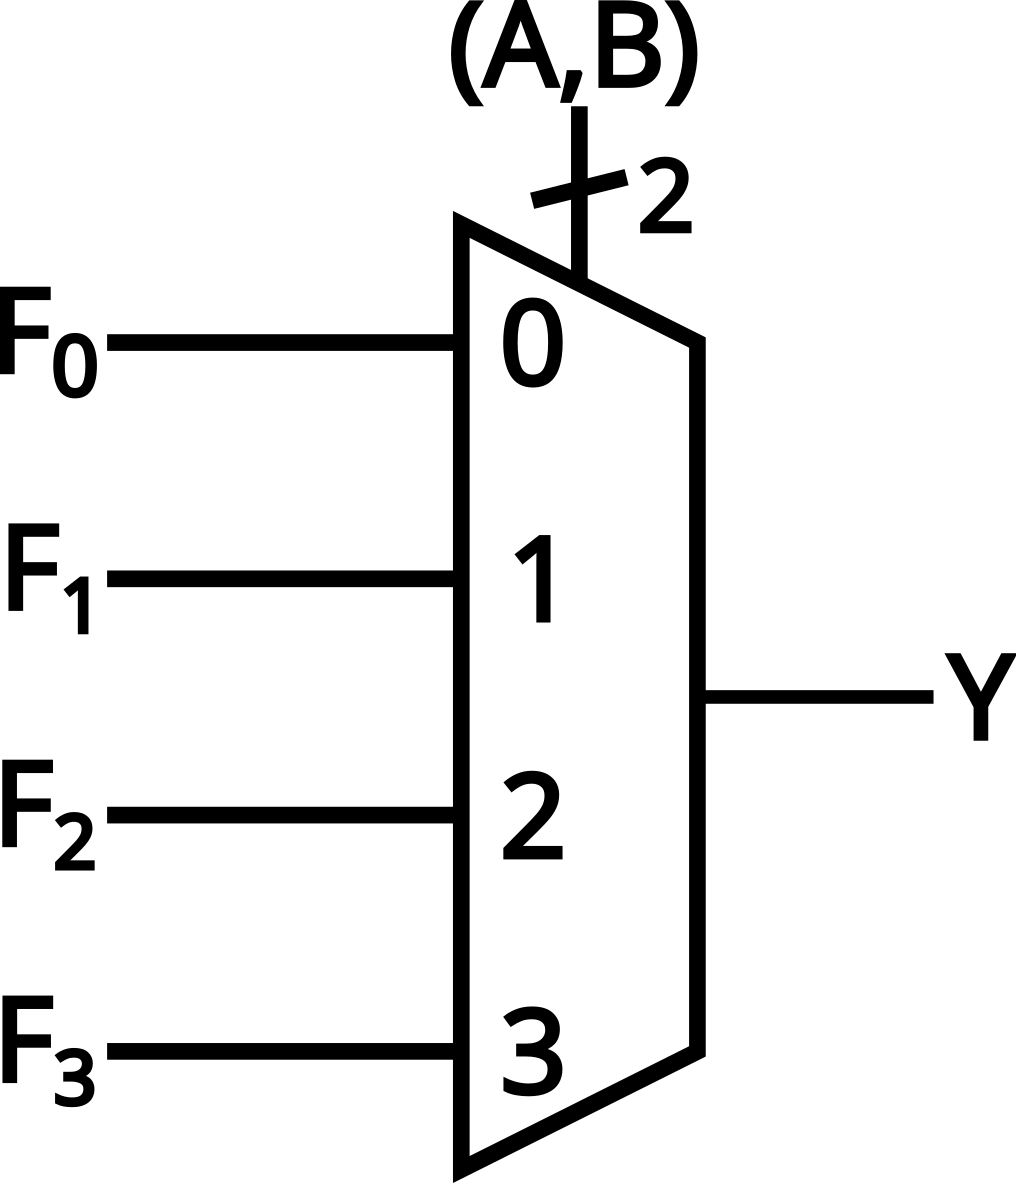
\includegraphics{Figures/MUX_Logic.png}
                    \caption{Wiring of a 4:1 mux as used in the logic section.}
                    \label{sec:ALU:MUXLogic:Logicer:MuxPic}
                \end{figure}


                This method is preferable when considering the number of ICs used:
                
                \begin{table}[htb]
                    \centering
                    \caption{Comparison of the number of components used in designs with (a) separate logic paths and (b) MUX-based logic}
                    \label{tab:ALU:MUXLogic:Logicer:NumICs}

                    \begin{subtable}{0.45\textwidth}
                        \centering
                        \begin{tabularx}{\textwidth}{
                            >{\hsize=0.40\hsize\arraybackslash}X
                            >{\hsize=0.30\hsize\arraybackslash}X
                            >{\hsize=0.25\hsize\arraybackslash}X
                            }

                            \addlinespace \toprule

                            Section     &\#Gates    &\#ICs  \\  \midrule

                            AND         &64         &16     \\
                            OR          &64         &16     \\
                            XOR         &64         &16     \\
                            4:1 MUX     &64         &32     \\  \midrule
                            Total       &256        &80     
                            
                        \end{tabularx}
                        \caption{Using discreet logic gates}

                    \end{subtable}
                    \hfill
                    \begin{subtable}{0.50\textwidth}
                        \centering
                        \begin{tabularx}{\textwidth}{
                            >{\hsize=0.5\hsize\arraybackslash}X
                            >{\hsize=0.25\hsize\arraybackslash}X
                            >{\hsize=0.25\hsize\arraybackslash}X
                            }

                            \addlinespace \toprule

                            Section     &\#Parts    &\#ICs  \\  \midrule

                            ROM Select  &1          &1      \\
                            ROM Diodes  &6          &---    \\
                            ROM Buffers &12         &2      \\
                            4:1 MUX     &64         &32     \\  \midrule
                            Total       &75         &35     
                            
                        \end{tabularx}
                        \caption{Using MUXs}

                    \end{subtable}

                    
                \end{table}

            \subsubsection{Setting up the MUX}\label{sec:ALU:Logicer:MUXSetup}

                The correct truth table is sleected using a 2:4 selector which is wired
                    to a small, diode ROM (\cref{fig:ALU:Logicer:MUXSetup:MUX_ROM}).
                    A 74x1G139 2:4 takes the two-bit function select and the desired 
                    bits are set from \(F_0, F_1, F_2, F_3\), which are then buffered
                    before being sent out to the MUXs. The unused decoder output is left 
                    unconnected and results in a fixed output of 0.

                \begin{figure}[htb]
                    \centering
                    \begin{circuitikz}\ctikzset{bipoles/length=1cm, nodes width=0.1}
                        %Vertical lines
                        \draw (1, 5) to (1, 0);
                        \draw (3, 5) to (3, 0);
                        \draw (5, 5) to (5, 0);
                        %Vertical Labels
                        \node[anchor=south](AND_Lab) at (1, 5) {\Large AND};
                        \node[anchor=south](OR_Lab) at (3, 5) {\Large OR};
                        \node[anchor=south](XOR_Lab) at (5, 5) {\Large XOR};
                        
                        %Horizontal lines
                        \draw (0, 4) to (7, 4);
                        \draw (0, 3) to (7, 3);
                        \draw (0, 2) to (7, 2);
                        \draw (0, 1) to (7, 1);
                        %Horizontal Labels
                        \node[anchor=east](F0_Lab) at (0, 4) {\Large\(F_0\)};
                        \node[anchor=east](F0_Lab) at (0, 3) {\Large\(F_1\)};
                        \node[anchor=east](F0_Lab) at (0, 2) {\Large\(F_2\)};
                        \node[anchor=east](F0_Lab) at (0, 1) {\Large\(F_3\)};

                        %Draw Buffers
                        \draw (7, 1) node[ieeestd buffer port, anchor=in 1]{};
                        \draw (7, 2) node[ieeestd buffer port, anchor=in 1]{};
                        \draw (7, 3) node[ieeestd buffer port, anchor=in 1]{};
                        \draw (7, 4) node[ieeestd buffer port, anchor=in 1]{};

                        %Draw Diodes
                        %AND
                        \draw (1, 1.5) to [full Schottky diode] (2, 1);

                        %OR
                        \draw (3, 3.5) to [full Schottky diode] (4, 3);
                        \draw (3, 2.5) to [full Schottky diode] (4, 2);
                        \draw (3, 1.5) to [full Schottky diode] (4, 1);

                        %XOR
                        \draw (5, 3.5) to [full Schottky diode] (6, 3);
                        \draw (5, 2.5) to [full Schottky diode] (6, 2);

                    \end{circuitikz}
                    \caption{Diode ROM storing the truth table function, \(F_0, F_1, F_2, F_3\).
                                Pull down resistors on all \(F_n\) lines omitted for clarity.}
                    \label{fig:ALU:Logicer:MUXSetup:MUX_ROM}
                \end{figure}

                As there are 64 total MUXs needed for the logic functions, the 
                    \emph{Function} lines are buffered four times in parallel, so each 
                    buffer only needs to drive 16 inputs. The buffers are needed at all 
                    both because of the high fanout requirement and because of the forward 
                    bias of the Schottkey diodes. With a forward drop of approx. 0.3 V; 
                    this drops the nominal signal level to 3.0 V, only 0.6 V above the
                    minimum \(V_{ih}\) of low-voltage CMOS logic chips.

        \subsection{Shifter}\label{sec:ALU:Shifter}

            The RISC-V ISA defines several shift operations, each of which can, in one
                operation, shift the input by an arbitrary number of bits up to X\_LEN-1.
                In RV64i, additional instructions shift 32-bit values and sign extend
                up to 64-bits. Both left and right shifts are defined, with left shifts
                being implemented by reversing the input, shifting, then reversing the
                result again:

                \begin{equation}\label{eq:ALU:Shifter:RevShift}
                    A >> B := \text{REV}(\ \text{REV}(A) << B \ )
                \end{equation}

            This implementation favours left shifts, so any rightward shift will use
                the method in \cref{eq:ALU:Shifter:RevShift}.

            Shifts are implemented using a sequential barrel shifter - a series
                of stages which shift the input a power of two number of places
                up to 32. Each stage consists of two tri-state buffers, one buffering
                the previous stage as is, the other buffering the previous output shifted
                by the next number of bits. The \(n^{th}\) stage is then controlled by
                the \(n^{th}\) bit of the shift amount input. 
                
            Traditionally, a sequential barrel shifter like this would use multiplexers, 
                but this requires far too many (384 MUXs across 96 ICs) to be practical. 
                The modified version using buffers comes from R. Baruch's RISC-V build
                \cite{RobB_Shifter}, expanded to 64-bits.
                
            Using 16-bit buffers in the 74LVC162244, the number of ICs can be reduced to 
                8 per stage, for a total of 48 - half that of the MUX version.

            \subsubsection{Bit Order Reverser}\label{sec:ALU:Shifter:BitRev}

                In order to shift the incoming number, \textbf{A}, rightwards, it must
                    be bit-reversed first. This is accomplished using two tri-state
                    buffers, one buffering the number as is, the other buffering the
                    reversed number.
                
                The reversal is accomplished by "simple" shuffling of the order of traces
                    on the PCB in the folowing way:

                [DIAGRAM OF PCB TRACE REVERSAL]

            \subsubsection{Shift Stages}\label{sec:ALU:Shifter:ShiftStages}


            

            

    \printbibliography[heading=bibintoc, title={References}]
\end{document}